\documentclass{standalone}
\usepackage{tikz}
\usepackage{pgfplots}
\pgfplotsset{compat=1.16}

\begin{document}
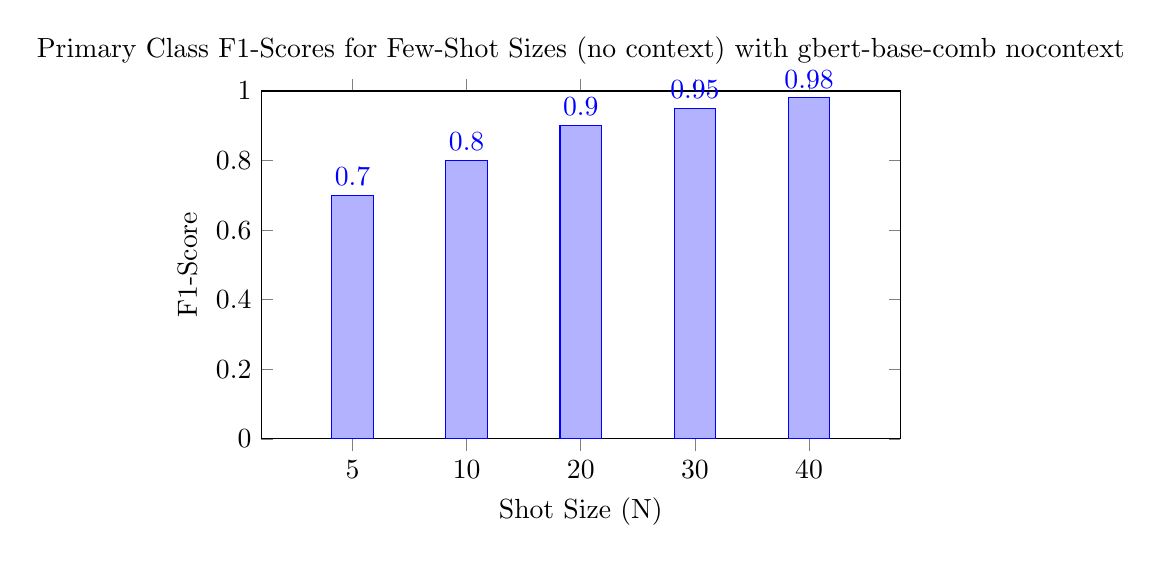
\begin{tikzpicture}
    \begin{axis}[
        ybar,
        symbolic x coords={5, 10, 20, 30, 40},
        xtick=data,
        nodes near coords,
        nodes near coords align={vertical},
        ylabel={F1-Score},
        xlabel={Shot Size (N)},
        title={Primary Class F1-Scores for Few-Shot Sizes (no context) with gbert-base-comb nocontext},
        width=0.8\textwidth,
        height=6cm,
        bar width=15pt,
        ymin=0,
        ymax=1,
        enlarge x limits=0.2
    ]
        \addplot coordinates {(5, 0.7) (10, 0.8) (20, 0.9) (30, 0.95) (40, 0.98)};
    \end{axis}
\end{tikzpicture}
\end{document}